\section{Auswertung}
\label{sec:Auswertung}
Um aus den Messwerten aus dem Refektivitätsscan Schichtdicke, Dispersion
und Rauigkeit der Polysterolschicht sowie Dispersion und Rauigkeit des Siliziumwafers
zu ermitteln, wird
% Untergrund von Messung mit Probe abziehen
zu Beginn der diffuse Scan von den Messwerten abgezogen wie in Abbildung
\ref{fig:diffuse_Scan} zu sehen.

\begin{figure}
  \centering
  \includegraphics[width=0.7\textwidth]{build/plot_messung_untergrund}
  \caption{Reflektivitätsscan und diffuser Scan und die Differenz von Reflektivitätsscan und diffuser Scan.}
  \label{fig:diffuse_Scan}
\end{figure}

Da erst ab einem ausreichend großen Einfallswinkel,
dem so definierte Geometriewinkel $\alpha_g$,
der gesamte Strahl auf die Oberfläche trifft,
werden die Messwerte mit $\alpha_i < \alpha_g$
mit einem Geometriefaktor $G$ korrigiert.
Dieser berücksichtigt den Intensitätsverlust, da
nicht der gesamte Strahl von der Probe reflektiert wird.
Der Geometriefaktor ergibt sich somit zu
\begin{align}
G&=\frac{D\sin\alpha_i}{d_0} &  &\text{für} \alpha_i<\alpha_g \\
G&=1 & &\text{für} \alpha_i<\alpha_g
\end{align}
mit der Gesamtstrahlbreite $d_0$ und der Durchmesser der Probenoberfläche $D$.
Ein Beispielhafter Strahlenverlauf für $\alpha_i<\alpha_g$ ist in Abbildung \ref{fig:geo}
dargestellt.
\begin{figure}
  \centering
  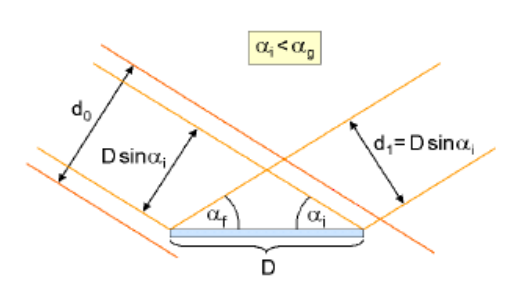
\includegraphics{bilder/geo_winkel.PNG}
  \caption{Strahlenverlauf für $\alpha_i<\alpha_g$. \cite{sample}}
  \label{fig:geo}
\end{figure}

Der Strahldurchmesser $d_0$ und der Druchmesser der Probenoberfläche $D$
ergeben sich aus den Messungen die zur Justage zwecken vor der eigentlichen Messung durchgeführt werden.
Aus dem Messwerten des Detektorscan ergibt sich der in Abbildung \ref{fig:det_scan}
gezeigte Intensitätsverlauf in Abhängigkeit des Detektorwinkel $\Theta'$.
\begin{figure}
  \centering
  \includegraphics[width=0.7\textwidth]{build/plot_det_scan.pdf}
  \caption{Intensität in Abhängigkeit des Detektorwinkels $\Theta'$ während eines Detektorscans und Fit an die Intensitätsverteilung.}
  \label{fig:det_scan}
\end{figure}

Durch einen Fit der Form
\begin{align}
I(\Theta) =  a \exp\left(-\frac{(\Theta-\mu)^2}{\omega^2}\right) \text{\cite{wiki_strahl}}
\end{align}
an die Intensitätsverteilung ergibt sich für den Strahldurchmesser

\begin{align}
d_0 = 2 \sin(\omega) R \label{eqn:d_o}
\end{align}
mit dem Radius $R$ des Detektorschiene.
Für die Fitparameter
\begin{align}
\mu&= & \omega&= \\
\end{align}
und dem Radius $R=\SI{0.5}{\meter}$?? folgt für den Strahldurchmesser
\begin{align}
  d_0=\SI{}{\meter}.
\end{align}

Zur Ermittelung der Probenoberfläche $D$ wird zunächst aus den Messwerten
des Rockingscan mit $2\Theta = \SI{0}{\degree}$, die in der Abblidung \ref{fig:rock_scan_0}
dargestellt sind,
der Geometriewinkel  $\alpha_g$ bestimmt.


\begin{figure}
  \centering
  \includegraphics[width=0.7\textwidth]{build/plot_rocking.pdf}
  \caption{Messwerte des Rockingscan mit $2\Theta = \SI{0}{\degree}$ und Fit.}
  \label{fig:rock_scan_0}
\end{figure}

Dafür wird eine Funktion der Form
\begin{align}
  f(x) = a \lvert x + b \rvert + c
\end{align}
an die Messwerte angepasst und es ergeben sich die Parametern
\begin{align}
a&= &b&=  &c&=.
\end{align}
Dabei entspricht der Parameter $b$ nur einer fehlende Eichung in der Messung und
es wird für die Berechung des Geometriewinkels $b=0$ gesetzt.
Der Geometriewinkel entspricht dem Winkel, ab dem der Strahl
vollständig auf die Probe trifft. Bei dem Rockingscan für $2\Theta=\SI{0}{\degree}$
entspricht der Geometriewinkel genau dem Winkel ab dem keine Intensität
mehr auf den Detektor fällt und somit genau dem Betrag der Nullstellen der an die Messwerte
angepassten Funktion.
Der bestimmte Geometriewinkel $\alpha_g$
lautet
\begin{align}
\alpha_g = \lvert \pm\frac{c}{a} \rvert = \SI{0.48(1)}{\degree}.
\end{align}
Über den Zusammenhang
\begin{align}
D = d_0\sin(\alpha_g)
\end{align}
ergibt sich der Druchmesser
der Probenoberfläche.
\begin{align}
  D=\Si{}{\meter}
\end{align}
Die Messwerte $I_{\mathrm{mess}}$ mit $\alpha_i < \alpha_g $ werden mit dem Geometriefaktor $G$
in der Form
\begin{align}
  I_{\mathrm{korr}} = \frac{I_{\mathrm{mess}}}{G}
\end{align}
korrigiert. Die Korrigierten Messwerte mit Hilfe des Geometriefaktors sind in der Abbildung \ref{fig:korr} dargestellt.
\begin{figure}
  \centering
  \includegraphics[width=0.7\textwidth]{build/Geometriefaktor.pdf}
  \caption{$I_{\mathrm{mess}}$ und $I_{\mathrm{korr}}$ in Abhängigkeit des Einfallswinkel $\alpha_i$.}
  \label{fig:korr}
\end{figure}

Ebenfalls in der Abbildung \ref{fig:korr}
sind die lokalenminima im Refektivitätsscan markiert.
Über den Zusammenhang
\begin{align}
  
\end{align}
% Geometriewinkel aus daten von Justierung -> Korrekturfaktor G
% -> Daten korrigieren


% Schichtdicke mit formel (9)
% Dispersionsprofil mit Parrot Alg. ( Lage des krit. Winkels anpassen)
% (modifizierte Fresnel Koeff.fuer Rauigkeit)
% restliche Parameter



%
% \begin{figure}
%   \centering
%   \includegraphics{plot.pdf}
%   \caption{Plot.}
%   \label{fig:plot}
% \end{figure}
